\newpage
\subsection{Caso d'uso UC14: Amministrazione applicazione web}
\label{UC14}
\begin{figure}[ht]
	\centering
	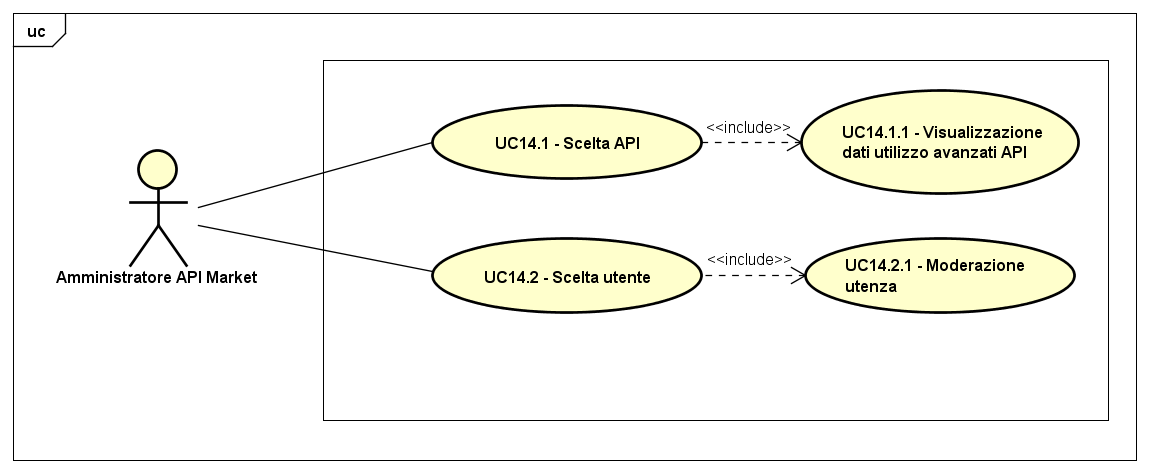
\includegraphics[scale=0.45]{UML/UC14.png}
	\caption{UC14: Amministrazione applicazione web}
\end{figure}

\renewcommand*{\arraystretch}{1.6}
\begin{longtable}{ l | p{11cm}}
	\hline
	\rowcolor{Gray}
	\multicolumn{2}{c}{UC14: Amministrazione applicazione web} \\
	\hline
	\textbf{Attori} & Amministratore API Market \\
	\textbf{Descrizione} & L'attore può gestire la parte riservata della piattaforma, ed effettuare operazioni super-user su utenza, prodotti registrati e sulla piattaforma stessa \\
	\textbf{Pre-Condizioni} & L'attore visita la pagina relativa all'amministrazione della piattaforma API Market\\
	\textbf{Post-Condizioni}& L'attore ha effettuato le modifiche desiderate, o ha consultato i dati desiderati, all'interno della piattaforma\\
	\textbf{Scenario Principale} & \begin{enumerate*}[label=(\arabic*.),itemjoin={\newline}]
		\item L'attore può consultare i dati di utilizzo avanzati per un API (UC14.1)
		\item L'attore può moderare l'utenza predisponendo sospensioni (UC14.2)
	\end{enumerate*}\\
\end{longtable}


\subsubsection{Caso d'uso UC14.1: Visualizzazione dati di utilizzo avanzati}
\label{UC14_1}

\begin{minipage}{\linewidth}
	\begin{tabular}{ l | p{11cm}}
		\hline
		\rowcolor{Gray}
		\multicolumn{2}{c}{UC14.1 - Visualizzazione dati di utilizzo avanzati} \\
		\hline
		\textbf{Attori} &  Amministratore API Market \\
		\textbf{Descrizione} & L'attore visualizza nella schermata relativa ai dati di utilizzo dell'API \\
		\textbf{Pre-Condizioni} & L'attore ha selezionato la visualizzazione dati per un API \\
		\textbf{Post-Condizioni} & L'attore ha visualizzato i dati di utilizzo avanzati dell'API selezionata \\
		\textbf{Scenario Principale} & 
		\begin{enumerate*}[label=(\arabic*.),itemjoin={\newline}]
			\item L'attore può visualizzare il numero di licenze attive per l'API selezionata (UC7.7.1)
			\item L'attore può visualizzare il numero di chiamate giornaliere effettuate all'API selezionata (UC7.7.2)
			\item L'attore può visualizzare il tempo medio di utilizzo dell'API selezionata (UC7.7.3)
			\item L'attore può visualizzare il traffico medio giornaliero dell'API selezionata (UC7.7.4)
			\item L'attore può visualizzare la lista di utenti che hanno una licenza attiva (UC14.1.1)
			\item L'attore può visualizzare il tempo medio di risposta (UC14.1.2)
		\end{enumerate*}\\
	\end{tabular}
\end{minipage}

\paragraph{Caso d'uso UC14.1.1: Visualizzazione utenti attivi per API}
\label{UC14_1_1}

\begin{minipage}{\linewidth}
	\begin{tabular}{ l | p{11cm}}
		\hline
		\rowcolor{Gray}
		\multicolumn{2}{c}{UC14.1.1 - Visualizzazione utenti attivi per API} \\
		\hline
		\textbf{Attori} & Amministratore API Market \\
		\textbf{Descrizione} & L'attore visualizza una lista di utenti attivi per l'API selezionata \\
		\textbf{Pre-Condizioni} & L'attore ha selezionato un API per il quale visualizzare i dati di utilizzo avanzati\\
		\textbf{Post-Condizioni} & L'attore ha visualizzato la lista di licenze attive per l'API selezionata \\
		\textbf{Scenario Principale} & 
		\begin{enumerate*}[label=(\arabic*.),itemjoin={\newline}]
			\item L'attore può visualizzare il nome dell'utente (UC14.1.1.1)
			\item L'attore può visualizzare la durata della licenza (UC14.1.1.2)
		\end{enumerate*}\\
	\end{tabular}
\end{minipage}

\subparagraph{Caso d'uso UC14.1.1.1: Visualizzazione nome}
\label{UC14_1_1_1}

\begin{minipage}{\linewidth}
	\begin{tabular}{ l | p{11cm}}
		\hline
		\rowcolor{Gray}
		\multicolumn{2}{c}{UC14.1.1.1 - Visualizzazione nome} \\
		\hline
		\textbf{Attori} & Amministratore API Market \\
		\textbf{Descrizione} & L'attore può visualizzare il nome dell'utente interessato\\
		\textbf{Pre-Condizioni} & L'attore è nella schermata di visualizzazione degli utenti con licenza attiva per l'API selezionata\\
		\textbf{Post-Condizioni} & L'attore ha visualizzato il nome interessato \\
		\textbf{Scenario Principale} & 
		\begin{enumerate*}[label=(\arabic*.),itemjoin={\newline}]
			\item L'attore può visualizzare il nome dell'utente corrispondente
		\end{enumerate*}
	\end{tabular}
\end{minipage}

\subparagraph{Caso d'uso UC14.1.1.2: Visualizzazione durata residua licenza}
\label{UC14_1_1_2}

\begin{minipage}{\linewidth}
	\begin{tabular}{ l | p{11cm}}
		\hline
		\rowcolor{Gray}
		\multicolumn{2}{c}{UC14.1.1.2 -  Visualizzazione durata residua licenza} \\
		\hline
		\textbf{Attori} & Amministratore API Market \\
		\textbf{Descrizione} & L'attore può visualizzare la durata residua della licenza dell'utente interessato\\
		\textbf{Pre-Condizioni} & L'attore è nella schermata di visualizzazione degli utenti con licenza attiva per l'API selezionata\\
		\textbf{Post-Condizioni} & L'attore ha visualizzato la data di scadenza \\
		\textbf{Scenario Principale} & 
		\begin{enumerate*}[label=(\arabic*.),itemjoin={\newline}]
			\item L'attore può visualizzare la scadenza per l'utente visualizzato riguardante l'API selezionata
		\end{enumerate*}
	\end{tabular}
\end{minipage}

\paragraph{Caso d'uso UC14.1.2: Visualizzazione tempo medio di risposta}
\label{UC14_1_2}

\begin{minipage}{\linewidth}
	\begin{tabular}{ l | p{11cm}}
		\hline
		\rowcolor{Gray}
		\multicolumn{2}{c}{UC14.1.2 - Visualizzazione tempo medio di risposta} \\
		\hline
		\textbf{Attori} & Amministratore API Market \\
		\textbf{Descrizione} & L'attore visualizza il tempo medio di risposta per l'API selezionata \\
		\textbf{Pre-Condizioni} & L'attore ha selezionato un API per il quale visualizzare i dati di utilizzo avanzati\\
		\textbf{Post-Condizioni} & L'attore ha visualizzato il tempo medio di risposta per l'API selezionata \\
		\textbf{Scenario Principale} & 
		\begin{enumerate*}[label=(\arabic*.),itemjoin={\newline}]
			\item L'attore può visualizzare il tempo medio di risposta per l'API selezionata
		\end{enumerate*}\\
	\end{tabular}
\end{minipage}

\subsubsection{Caso d'uso UC14.2: Azioni utente}
\label{UC14_2}

\begin{minipage}{\linewidth}
	\begin{tabular}{ l | p{11cm}}
		\hline
		\rowcolor{Gray}
		\multicolumn{2}{c}{UC14.2 - Azioni utente} \\
		\hline
		\textbf{Attori} &  Amministratore API Market \\
		\textbf{Descrizione} & L'attore visualizza nella schermata relativa ai dati di utilizzo dell'API \\
		\textbf{Pre-Condizioni} & L'attore ha selezionato la visualizzazione dati per un API \\
		\textbf{Post-Condizioni} & L'attore ha visualizzato i dati di utilizzo avanzati dell'API selezionata \\
		\textbf{Scenario Principale} & 
		\begin{enumerate*}[label=(\arabic*.),itemjoin={\newline}]
			\item L'attore può inserire il nome di un utente su cui effettuare un azione (UC14.2.1)
			\item L'attore può sospendere l'utente selezionato (UC14.2.2)
			\item L'attore può sospendere i prelievi di denaro dal proprio conto per l'utente selezionato (UC14.2.3)
			\item L'attore può rimuovere una sospensione utente (UC14.2.4)
			\item L'attore può rimuovere la sospensione dei prelievi (UC14.2.5)
		\end{enumerate*}\\
		\textbf{Scenari Alternativi} & 
		\begin{enumerate*}[label=(\arabic*.),itemjoin={\newline}]
			\item L'attore riceve un messaggio d'errore qualora l'utente inserito non esista. Può dunque ritentare la procedura
		\end{enumerate*}\\
	\end{tabular}
\end{minipage}

\paragraph{Caso d'uso UC14.2.1: Inserimento username}
\label{UC14_2_1}

\begin{minipage}{\linewidth}
	\begin{tabular}{ l | p{11cm}}
		\hline
		\rowcolor{Gray}
		\multicolumn{2}{c}{UC14.2.1 - Inserimento username} \\
		\hline
		\textbf{Attori} & Amministratore API Market \\
		\textbf{Descrizione} & L'attore inserisce l'username di un utente sul quale effettuare operazioni \\
		\textbf{Pre-Condizioni} & L'attore ha scelto di effettuare azioni su un utente\\
		\textbf{Post-Condizioni} & L'attore ha inserito il nome di un utente \\
		\textbf{Scenario Principale} & 
		\begin{enumerate*}[label=(\arabic*.),itemjoin={\newline}]
			\item L'attore può inserire il nome di un utente
		\end{enumerate*}\\
	\end{tabular}
\end{minipage}

\paragraph{Caso d'uso UC14.2.2: Sospensione utente}
\label{UC14_2_2}

\begin{minipage}{\linewidth}
	\begin{tabular}{ l | p{11cm}}
		\hline
		\rowcolor{Gray}
		\multicolumn{2}{c}{UC14.2.2 - Sospensione utente} \\
		\hline
		\textbf{Attori} & Amministratore API Market \\
		\textbf{Descrizione} & L'attore può sospendere l'utente indicato \\
		\textbf{Pre-Condizioni} & L'attore ha inserito il nome utente da sospendere\\
		\textbf{Post-Condizioni} & L'attore ha sospeso un utente \\
		\textbf{Scenario Principale} & 
		\begin{enumerate*}[label=(\arabic*.),itemjoin={\newline}]
			\item L'attore può inserire la durata in giorni della sospensione (UC14.2.2.1)
			\item L'attore può confermare la scelta (UC14.2.2.2)
		\end{enumerate*}\\
	\end{tabular}
\end{minipage}

\newpage
\textbf{Da fare: UC14.2.3 e sottocasi, UC14.2.4 e sottocasi, UC14.2.5 e sottocasi, UC14.2.2.1, UC14.2.2.2}